
\documentclass[letterpaper,hide notes,xcolor={table,svgnames},pdftex,10pt]{beamer}
\def\showexamples{t}


%\usepackage[svgnames]{xcolor}

%% Demo talk
%\documentclass[letterpaper,notes=show]{beamer}

\usecolortheme{crane}
\setbeamertemplate{navigation symbols}{}

\usetheme{MyPittsburgh}
%\usetheme{Frankfurt}

%\usepackage{tipa}

\usepackage{hyperref}
\usepackage{graphicx,xspace}
\usepackage[normalem]{ulem}
\usepackage{multicol}

\newcommand\SF[1]{$\bigstar$\footnote{SF: #1}}

\usepackage[default]{sourcesanspro}
\usepackage[T1]{fontenc}

\newcounter{tmpnumSlide}
\newcounter{tmpnumNote}

% old question code
%\newcommand\question[1]{{$\bigstar$ \small \onlySlide{2}{#1}}}
% \newcommand\nquestion[1]{\ifdefined \presentationonly \textcircled{?} \fi \note{\par{\Large \textbf{?}} #1}}
% \newcommand\nanswer[1]{\note{\par{\Large \textbf{A}} #1}}


 \newcommand\mnote[1]{%
   \addtocounter{tmpnumSlide}{1}
   \ifdefined\showcues {~\tiny\fbox{\arabic{tmpnumSlide}}}\fi
   \note{\setlength{\parskip}{1ex}\addtocounter{tmpnumNote}{1}\textbf{\Large \arabic{tmpnumNote}:} {#1\par}}}

\newcommand\mmnote[1]{\note{\setlength{\parskip}{1ex}#1\par}}

%\newcommand\mnote[2][]{\ifdefined\handoutwithnotes {~\tiny\fbox{#1}}\fi
% \note{\setlength{\parskip}{1ex}\textbf{\Large #1:} #2\par}}

%\newcommand\mnote[2][]{{\tiny\fbox{#1}} \note{\setlength{\parskip}{1ex}\textbf{\Large #1:} #2\par}}

\newcommand\mquestion[2]{{~\color{red}\fbox{?}}\note{\setlength{\parskip}{1ex}\par{\Large \textbf{?}} #1} \note{\setlength{\parskip}{1ex}\par{\Large \textbf{A}} #2\par}\ifdefined \presentationonly \pause \fi}

\newcommand\blackboard[1]{%
\ifdefined   \showblackboard
  {#1}
  \else {\begin{center} \fbox{\colorbox{blue!30}{%
         \begin{minipage}{.95\linewidth}%
           \hspace{\stretch{1}} Some space intentionally left blank; done at the blackboard.%
         \end{minipage}}}\end{center}}%
         \fi%
}



%\newcommand\q{\tikz \node[thick,color=black,shape=circle]{?};}
%\newcommand\q{\ifdefined \presentationonly \textcircled{?} \fi}

\usepackage{listings}
\lstset{%
  keywordstyle=\bfseries,
  aboveskip=15pt,
  belowskip=15pt,
  captionpos=b,
  identifierstyle=\ttfamily,
  escapeinside={(*@}{@*)},
  stringstyle=\ttfamiliy,
  frame=lines,
  numbers=left, basicstyle=\scriptsize, numberstyle=\tiny, stepnumber=0, numbersep=2pt}

\usepackage{siunitx}
\newcommand\sius[1]{\num[group-separator = {,}]{#1}\si{\micro\second}}
\newcommand\sims[1]{\num[group-separator = {,}]{#1}\si{\milli\second}}
\newcommand\sins[1]{\num[group-separator = {,}]{#1}\si{\nano\second}}
\sisetup{group-separator = {,}, group-digits = true}

%% -------------------- tikz --------------------
\usepackage{tikz}
\usetikzlibrary{positioning}
\usetikzlibrary{arrows,backgrounds,automata,decorations.shapes,decorations.pathmorphing,decorations.markings,decorations.text}

\tikzstyle{place}=[circle,draw=blue!50,fill=blue!20,thick, inner sep=0pt,minimum size=6mm]
\tikzstyle{transition}=[rectangle,draw=black!50,fill=black!20,thick, inner sep=0pt,minimum size=4mm]

\tikzstyle{block}=[rectangle,draw=black, thick, inner sep=5pt]
\tikzstyle{bullet}=[circle,draw=black, fill=black, thin, inner sep=2pt]

\tikzstyle{pre}=[<-,shorten <=1pt,>=stealth',semithick]
\tikzstyle{post}=[->,shorten >=1pt,>=stealth',semithick]
\tikzstyle{bi}=[<->,shorten >=1pt,shorten <=1pt, >=stealth',semithick]

\tikzstyle{mut}=[-,>=stealth',semithick]

\tikzstyle{treereset}=[dashed,->, shorten >=1pt,>=stealth',thin]

\usepackage{ifmtarg}
\usepackage{xifthen}
\makeatletter
% new counter to now which frame it is within the sequence
\newcounter{multiframecounter}
% initialize buffer for previously used frame title
\gdef\lastframetitle{\textit{undefined}}
% new environment for a multi-frame
\newenvironment{multiframe}[1][]{%
\ifthenelse{\isempty{#1}}{%
% if no frame title was set via optional parameter,
% only increase sequence counter by 1
\addtocounter{multiframecounter}{1}%
}{%
% new frame title has been provided, thus
% reset sequence counter to 1 and buffer frame title for later use
\setcounter{multiframecounter}{1}%
\gdef\lastframetitle{#1}%
}%
% start conventional frame environment and
% automatically set frame title followed by sequence counter
\begin{frame}%
\frametitle{\lastframetitle~{\normalfont(\arabic{multiframecounter})}}%
}{%
\end{frame}%
}
\makeatother

\makeatletter
\newdimen\tu@tmpa%
\newdimen\ydiffl%
\newdimen\xdiffl%
\newcommand\ydiff[2]{%
    \coordinate (tmpnamea) at (#1);%
    \coordinate (tmpnameb) at (#2);%
    \pgfextracty{\tu@tmpa}{\pgfpointanchor{tmpnamea}{center}}%
    \pgfextracty{\ydiffl}{\pgfpointanchor{tmpnameb}{center}}%
    \advance\ydiffl by -\tu@tmpa%
}
\newcommand\xdiff[2]{%
    \coordinate (tmpnamea) at (#1);%
    \coordinate (tmpnameb) at (#2);%
    \pgfextractx{\tu@tmpa}{\pgfpointanchor{tmpnamea}{center}}%
    \pgfextractx{\xdiffl}{\pgfpointanchor{tmpnameb}{center}}%
    \advance\xdiffl by -\tu@tmpa%
}
\makeatother
\newcommand{\copyrightbox}[3][r]{%
\begin{tikzpicture}%
\node[inner sep=0pt,minimum size=2em](ciimage){#2};
\usefont{OT1}{phv}{n}{n}\fontsize{4}{4}\selectfont
\ydiff{ciimage.south}{ciimage.north}
\xdiff{ciimage.west}{ciimage.east}
\ifthenelse{\equal{#1}{r}}{%
\node[inner sep=0pt,right=1ex of ciimage.south east,anchor=north west,rotate=90]%
{\raggedleft\color{black!50}\parbox{\the\ydiffl}{\raggedright{}#3}};%
}{%
\ifthenelse{\equal{#1}{l}}{%
\node[inner sep=0pt,right=1ex of ciimage.south west,anchor=south west,rotate=90]%
{\raggedleft\color{black!50}\parbox{\the\ydiffl}{\raggedright{}#3}};%
}{%
\node[inner sep=0pt,below=1ex of ciimage.south west,anchor=north west]%
{\raggedleft\color{black!50}\parbox{\the\xdiffl}{\raggedright{}#3}};%
}
}
\end{tikzpicture}
}


%% --------------------

%\usepackage[excludeor]{everyhook}
%\PushPreHook{par}{\setbox0=\lastbox\llap{MUH}}\box0}

%\vspace*{\stretch{1}

%\setbox0=\lastbox \llap{\textbullet\enskip}\box0}

\setlength{\parskip}{\fill}

\newcommand\noskips{\setlength{\parskip}{1ex}}
\newcommand\doskips{\setlength{\parskip}{\fill}}

\newcommand\xx{\par\vspace*{\stretch{1}}\par}
\newcommand\xxs{\par\vspace*{2ex}\par}
\newcommand\tuple[1]{\langle #1 \rangle}
\newcommand\code[1]{{\sf \footnotesize #1}}
\newcommand\ex[1]{\uline{Example:} \ifdefined \presentationonly \pause \fi
  \ifdefined\showexamples#1\xspace\else{\uline{\hspace*{2cm}}}\fi}

\newcommand\ceil[1]{\lceil #1 \rceil}


\AtBeginSection[]
{
   \begin{frame}
       \frametitle{Outline}
       \tableofcontents[currentsection]
   \end{frame}
}



\pgfdeclarelayer{edgelayer}
\pgfdeclarelayer{nodelayer}
\pgfsetlayers{edgelayer,nodelayer,main}

\tikzstyle{none}=[inner sep=0pt]
\tikzstyle{rn}=[circle,fill=Red,draw=Black,line width=0.8 pt]
\tikzstyle{gn}=[circle,fill=Lime,draw=Black,line width=0.8 pt]
\tikzstyle{yn}=[circle,fill=Yellow,draw=Black,line width=0.8 pt]
\tikzstyle{empty}=[circle,fill=White,draw=Black]
\tikzstyle{bw} = [rectangle, draw, fill=blue!20, 
    text width=4em, text centered, rounded corners, minimum height=2em]
    
    \newcommand{\CcNote}[1]{% longname
	This work is licensed under the \textit{Creative Commons #1 3.0 License}.%
}
\newcommand{\CcImageBy}[1]{%
	\includegraphics[scale=#1]{creative_commons/cc_by_30.pdf}%
}
\newcommand{\CcImageSa}[1]{%
	\includegraphics[scale=#1]{creative_commons/cc_sa_30.pdf}%
}
\newcommand{\CcImageNc}[1]{%
	\includegraphics[scale=#1]{creative_commons/cc_nc_30.pdf}%
}
\newcommand{\CcGroupBySa}[2]{% zoom, gap
	\CcImageBy{#1}\hspace*{#2}\CcImageNc{#1}\hspace*{#2}\CcImageSa{#1}%
}
\newcommand{\CcLongnameByNcSa}{Attribution-NonCommercial-ShareAlike}

\newenvironment{changemargin}[1]{% 
  \begin{list}{}{% 
    \setlength{\topsep}{0pt}% 
    \setlength{\leftmargin}{#1}% 
    \setlength{\rightmargin}{1em}
    \setlength{\listparindent}{\parindent}% 
    \setlength{\itemindent}{\parindent}% 
    \setlength{\parsep}{\parskip}% 
  }% 
  \item[]}{\end{list}} 




\title{Lecture 1 --- Introduction, Law, \& Justice}

\author{Jeff Zarnett \\ \small \texttt{jzarnett@uwaterloo.ca}}
\institute{Department of Electrical and Computer Engineering \\
  University of Waterloo}
\date{\today}


\begin{document}

\begin{frame}
  \titlepage

\begin{center}
  \small{Acknowledgments: Douglas Harder~\cite{dwh}, Julie Vale~\cite{jv}}
  \end{center}
\end{frame}


\begin{frame}
\frametitle{Course Syllabus}

As our first order of business, let's go over the course syllabus.

\end{frame}

\begin{frame}
\frametitle{Collaborative Course}

The source material for the ECE~290 notes and slides is now open-sourced via Github. 

If you find an error in the notes/slides, or have an improvement, go to \url{https://github.com/jzarnett/ece290} and open an issue. 

If you know how to use \texttt{git} and \LaTeX, then you can go to the URL and submit a pull request (changes) for me to look at and incorporate!


\end{frame}



\begin{frame}
\frametitle{Law}

The law is a complex subject and ``Law'' does not have a concise definition.

Example 1 from~\cite{lba}: Mary Brown is at home with her 18-month old baby. The baby is ill and has a fever.

Ms. Brown discovers the baby has fallen into a coma. Fearing for his life, she gets in her car and rushes the child to the hospital.

On the way to the hospital, she drives 115 km/h in a 50 km/h zone. 

At the hospital, a doctor commends Ms. Brown for saving the life of her child.

A policeman presents Ms. Brown with a summons for dangerous driving.

\end{frame}



\begin{frame}
\frametitle{The Case of Ms. Brown}

Ms. Brown drove her car far above the speed limit.\\
\quad Clearly, she broke the law.

She endangered the lives of others (drivers, cyclists, pedestrians).\\
\quad But she also saved the life of her child.

Were her actions justified? Reasonable?

What will she say in court about her charge of dangerous driving?

What is the court likely to do?

\end{frame}



\begin{frame}
\frametitle{Hard Questions}

This leads us to some hard questions:

\begin{itemize}
	\item Why should we obey laws?
	\item Is it ever right to obey a law?
	\item Is law the same thing as justice? 
	\item What is justice?
\end{itemize}


\end{frame}


\begin{frame}
\frametitle{What is Justice?}

\begin{center}

\includegraphics[width=0.8\textwidth]{images/justiceleague-dinei.jpg}
\end{center}
{\scriptsize Source: \url{http://dinei.deviantart.com/art/the-Justice-League-of-America-of-the-Benes-336058471}}

\end{frame}


\begin{frame}
\frametitle{Justice}

A potential definition of justice:

\begin{quote}
The quality of being (morally) just or righteous; the principle of just dealing; the exhibition of this quality or principle in action; just conduct; integrity, rectitude. (One of the four cardinal virtues.)
\end{quote}

\end{frame}

\begin{frame}
\frametitle{Justice}

A potential definition of justice:

\begin{quote}
Conformity (of an action or thing) to moral right, or to reason, truth, or fact; rightfulness; fairness; correctness; propriety
\end{quote}

\end{frame}

\begin{frame}
\frametitle{Justice}

A potential definition of justice:

\begin{quote}
Exercise of authority or power in maintenance of right; vindication of right by assignment of reward or punishment; requital of desert.

\end{quote}

\end{frame}

\begin{frame}
\frametitle{Justice}

A potential definition of justice:

\begin{center}
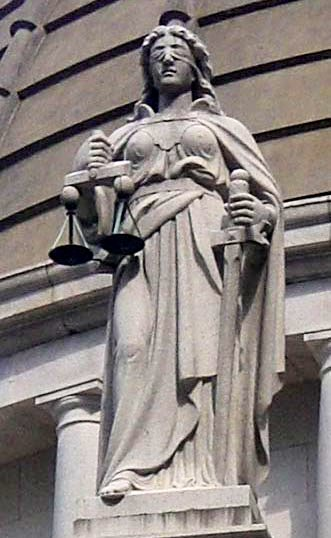
\includegraphics[width=0.2\textwidth]{images/lady-justice.jpg}\\
{\scriptsize \textit{Justicia}, Court of Final Appeal, Hong Kong.\footnote{Source: By ChvhLR10 - Own work, CC BY-SA 3.0, \url{https://commons.wikimedia.org/w/index.php?curid=4707069}}}
\end{center}


\begin{quote}
Personified often represented in art as a goddess holding balanced scales or a sword, sometimes also with veiled eyes, betokening impartiality.
\end{quote}

\end{frame}



\begin{frame}
\frametitle{Other Definitions}

Plato defined justice as \textit{harmony}.

There is also \textit{Divine Command Theory} -- justice stems from a divine authority.

Natural law: a rational person applying reason and logic will arrive at some basic principles of justice.


\end{frame}



\begin{frame}
\frametitle{Laws of Nature and Laws of Man}

The word ``law'' is used frequently in your engineering education to refer to laws of nature: e.g., Newton's Third \textit{Law} of Motion.

The second meaning of the law refers to rules governing conduct~\cite{lba}.

A law that forbids stealing does not make it physically impossible to steal.\\
\quad It says one should not steal and that there are consequences for doing so.

This is a \alert{normative} law rather than a \alert{physical} law.

One can break a normative law, and risk the consequences.

\end{frame}



\begin{frame}
\frametitle{Theory of Social Contract}

The theory of social contract says that laws are a collective agreement.

People surrender some rights and freedoms to the state.

In return they receive protection of the remaining rights and freedoms.

Covenants with divine beings stretch back to antiquity.

\end{frame}



\begin{frame}
\frametitle{Alternate Definition of Justice}

Another way to think about justice:

\begin{quote}
	Justice is the preservation of property and keeping of agreements.
\end{quote}

\end{frame}



\begin{frame}
\frametitle{Branches of Justice}

Justice itself is complicated and takes several forms.

\begin{center}
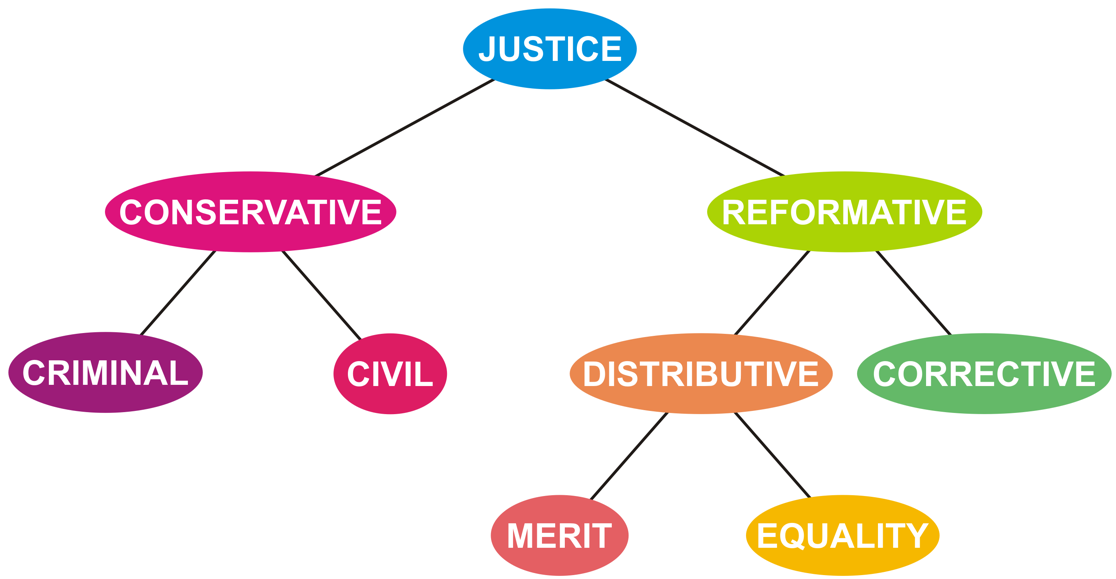
\includegraphics[width=0.8\textwidth]{images/justice-branches.png}\\
{\scriptsize Image Credit: D. W. Harder}
\end{center}


\end{frame}



\begin{frame}
\frametitle{Conservative Justice}

One goal of justice is to \alert{conserve} the state of society.

Like the TV show suggests, law and order go hand in hand.

The state creates and maintains laws.

\end{frame}



\begin{frame}
\frametitle{Criminal Justice}

Criminal justice defines what is a crime: an action that constitutes an offence and will be prosecuted and punished.

In a criminal case, the ``wronged'' party is the state (in Canada, the Crown).

The state (the crown) initiates legal proceedings.

Criminal justice seeks to maintain the society as a whole.

Its goals are:
\begin{itemize}
\item Deter and mitigate crime
\item Penalize and rehabilitate offenders
\end{itemize}

Sometimes called retributive justice.

This is the kind of thing you see on \textit{Law \& Order}.

\end{frame}



\begin{frame}
\frametitle{Civil Justice}

Civil justice regulates actions between individuals.

The party who is ``wronged'' must initiate legal proceedings.

The goal of civil justice is \alert{restorative}: restore the injured party, to the extent possible, to its original state.

TV Shows like \textit{People's Court} or (dare I say it) \textit{Judge Judy}.

\end{frame}



\begin{frame}
\frametitle{Reform Society}

Another aspect of justice is to reform society.

Traditionally, this includes incarceration and other forms of punishment.

Imprisonment was not considered a punishment in itself until recent history.

Instead, it hold the individual until punishment was administered.

Punishment was often quite severe (e.g., forced amputation!).

\end{frame}



\begin{frame}
\frametitle{Restorative Justice}

In recent years there has been an increase in restorative rather than punitive justice.

Some examples:

\begin{itemize}
\item Victim-offender mediation
\item Family group or community conferencing and boards
\item Community restorative boards
\item Sentencing circles
\end{itemize}

\end{frame}



\begin{frame}
\frametitle{Distributive Justice}
This involves the \textit{just} allocation of goods in society.

Distribution can be decided through:
\begin{itemize}
	\item Equity
	\item Equality
	\item Power
	\item Need
	\item Responsibility
\end{itemize}

\end{frame}



\begin{frame}
\frametitle{John Rawls' Theory of Justice}

John Rawls wrote a book \textit{A Theory of Justice}.

In it, he equates justice with fairness.

How do we set up guidelines for what is fair?


\end{frame}



\begin{frame}
\frametitle{John Rawls' Theory of Justice}

Key idea: \alert{The veil of ignorance}.

Create guidelines for society under the assumption you are not aware of what position you will take within that society.


Social and economic inequalities must conform to:
\begin{itemize}
\item They must be of most advantage to the least advantaged in society
\item Public offices and positions must be open to everyone under conditions of fair equality of opportunity
\end{itemize}


\end{frame}



\begin{frame}
\frametitle{Purpose of the Legal System}

The legal system is expected to deliver the forms of justice we have discussed.

Society only functions if people obey the law:
\begin{itemize}
\item Workers won't work if they think their employer won't pay their wages.
\item People won't trade goods if they can be cheated without consequence.
\item If criminals are not punished, people take the law into their own hands...
\end{itemize}


\end{frame}



\begin{frame}
\frametitle{Purpose of the Legal System}

\begin{quote}
A legal system provides the broad framework for the detailed rules that create the essential qualities of a stable society. If men feel free to either obey or break the rules as they wish, then the rules will not secure the minimum standards of peace and predictability. We may conclude, therefore, that citizens generally ought to obey the law because in doing so they promote a reasonably harmonious society. If a legal system is to encourage most men to accept this view, it must appear to them to be generally just...
\end{quote}
\hfill~\cite{lba}

\end{frame}


\begin{frame}
\frametitle{References \& Disclaimer}
\bibliographystyle{alphaurl}
\setbeamertemplate{bibliography item}{\insertbiblabel}
{\scriptsize
\bibliography{290}
}
\vfill

{\tiny Disclaimer: the material presented in these lectures slides is intended for use in the course ECE~290 at the University of Waterloo and should not be relied upon as legal advice. Any reliance on these course slides by any party for any other purpose are the responsibility of such parties.  The author(s) accept(s) no responsibility for damages, if any, suffered by any party as a result of decisions made or actions based on these course slides for any other purpose than that for which it was intended.\par}


\end{frame}


\end{document}

